\section{RTC::Execution\-Context\-Service Interface Reference}
\label{interfaceRTC_1_1ExecutionContextService}\index{RTC::ExecutionContextService@{RTC::ExecutionContextService}}
Introspection::Execution\-Context\-Service interface.  


{\tt import \char`\"{}RTC.idl\char`\"{};}

Inheritance diagram for RTC::Execution\-Context\-Service::\begin{figure}[H]
\begin{center}
\leavevmode
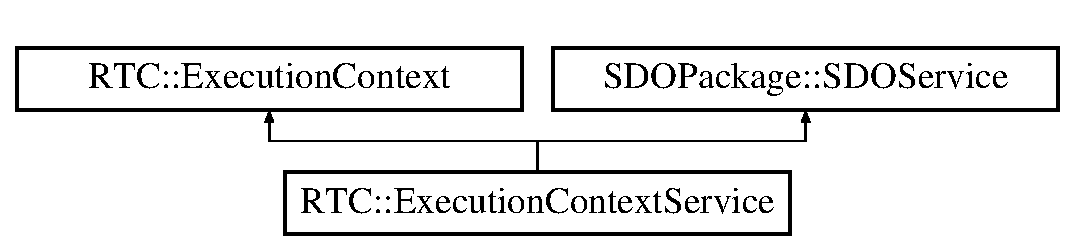
\includegraphics[height=2cm]{interfaceRTC_1_1ExecutionContextService}
\end{center}
\end{figure}
\subsection*{Public Member Functions}
\begin{CompactItemize}
\item 
{\bf Execution\-Context\-Profile} {\bf get\_\-profile} ()
\item 
boolean {\bf is\_\-running} ()
\item 
{\bf Return\-Code\_\-t} {\bf start} ()
\item 
{\bf Return\-Code\_\-t} {\bf stop} ()
\item 
double {\bf get\_\-rate} ()
\item 
{\bf Return\-Code\_\-t} {\bf set\_\-rate} (in double rate)
\item 
{\bf Return\-Code\_\-t} {\bf activate\_\-component} (in {\bf Lightweight\-RTObject} comp)
\item 
{\bf Return\-Code\_\-t} {\bf deactivate\_\-component} (in {\bf Lightweight\-RTObject} comp)
\item 
{\bf Return\-Code\_\-t} {\bf reset\_\-component} (in {\bf Lightweight\-RTObject} comp)
\item 
{\bf Life\-Cycle\-State} {\bf get\_\-component\_\-state} (in {\bf Lightweight\-RTObject} comp)
\item 
{\bf Execution\-Kind} {\bf get\_\-kind} ()
\item 
{\bf Return\-Code\_\-t} {\bf add} (in {\bf Lightweight\-RTObject} comp)
\item 
{\bf Return\-Code\_\-t} {\bf remove} (in {\bf Lightweight\-RTObject} comp)
\end{CompactItemize}


\subsection{Detailed Description}
Introspection::Execution\-Context\-Service interface. 



\subsection{Member Function Documentation}
\index{RTC::ExecutionContextService@{RTC::Execution\-Context\-Service}!activate_component@{activate\_\-component}}
\index{activate_component@{activate\_\-component}!RTC::ExecutionContextService@{RTC::Execution\-Context\-Service}}
\subsubsection{\setlength{\rightskip}{0pt plus 5cm}{\bf Return\-Code\_\-t} RTC::Execution\-Context::activate\_\-component (in {\bf Lightweight\-RTObject} {\em comp})\hspace{0.3cm}{\tt  [inherited]}}\label{interfaceRTC_1_1ExecutionContext_RTC_1_1ExecutionContextServicea6}


\index{RTC::ExecutionContextService@{RTC::Execution\-Context\-Service}!add@{add}}
\index{add@{add}!RTC::ExecutionContextService@{RTC::Execution\-Context\-Service}}
\subsubsection{\setlength{\rightskip}{0pt plus 5cm}{\bf Return\-Code\_\-t} RTC::Execution\-Context::add (in {\bf Lightweight\-RTObject} {\em comp})\hspace{0.3cm}{\tt  [inherited]}}\label{interfaceRTC_1_1ExecutionContext_RTC_1_1ExecutionContextServicea11}


\index{RTC::ExecutionContextService@{RTC::Execution\-Context\-Service}!deactivate_component@{deactivate\_\-component}}
\index{deactivate_component@{deactivate\_\-component}!RTC::ExecutionContextService@{RTC::Execution\-Context\-Service}}
\subsubsection{\setlength{\rightskip}{0pt plus 5cm}{\bf Return\-Code\_\-t} RTC::Execution\-Context::deactivate\_\-component (in {\bf Lightweight\-RTObject} {\em comp})\hspace{0.3cm}{\tt  [inherited]}}\label{interfaceRTC_1_1ExecutionContext_RTC_1_1ExecutionContextServicea7}


\index{RTC::ExecutionContextService@{RTC::Execution\-Context\-Service}!get_component_state@{get\_\-component\_\-state}}
\index{get_component_state@{get\_\-component\_\-state}!RTC::ExecutionContextService@{RTC::Execution\-Context\-Service}}
\subsubsection{\setlength{\rightskip}{0pt plus 5cm}{\bf Life\-Cycle\-State} RTC::Execution\-Context::get\_\-component\_\-state (in {\bf Lightweight\-RTObject} {\em comp})\hspace{0.3cm}{\tt  [inherited]}}\label{interfaceRTC_1_1ExecutionContext_RTC_1_1ExecutionContextServicea9}


\index{RTC::ExecutionContextService@{RTC::Execution\-Context\-Service}!get_kind@{get\_\-kind}}
\index{get_kind@{get\_\-kind}!RTC::ExecutionContextService@{RTC::Execution\-Context\-Service}}
\subsubsection{\setlength{\rightskip}{0pt plus 5cm}{\bf Execution\-Kind} RTC::Execution\-Context::get\_\-kind ()\hspace{0.3cm}{\tt  [inherited]}}\label{interfaceRTC_1_1ExecutionContext_RTC_1_1ExecutionContextServicea10}


\index{RTC::ExecutionContextService@{RTC::Execution\-Context\-Service}!get_profile@{get\_\-profile}}
\index{get_profile@{get\_\-profile}!RTC::ExecutionContextService@{RTC::Execution\-Context\-Service}}
\subsubsection{\setlength{\rightskip}{0pt plus 5cm}{\bf Execution\-Context\-Profile} RTC::Execution\-Context\-Service::get\_\-profile ()}\label{interfaceRTC_1_1ExecutionContextService_RTC_1_1ExecutionContextServicea0}


\index{RTC::ExecutionContextService@{RTC::Execution\-Context\-Service}!get_rate@{get\_\-rate}}
\index{get_rate@{get\_\-rate}!RTC::ExecutionContextService@{RTC::Execution\-Context\-Service}}
\subsubsection{\setlength{\rightskip}{0pt plus 5cm}double RTC::Execution\-Context::get\_\-rate ()\hspace{0.3cm}{\tt  [inherited]}}\label{interfaceRTC_1_1ExecutionContext_RTC_1_1ExecutionContextServicea4}


\index{RTC::ExecutionContextService@{RTC::Execution\-Context\-Service}!is_running@{is\_\-running}}
\index{is_running@{is\_\-running}!RTC::ExecutionContextService@{RTC::Execution\-Context\-Service}}
\subsubsection{\setlength{\rightskip}{0pt plus 5cm}boolean RTC::Execution\-Context::is\_\-running ()\hspace{0.3cm}{\tt  [inherited]}}\label{interfaceRTC_1_1ExecutionContext_RTC_1_1ExecutionContextServicea1}


\index{RTC::ExecutionContextService@{RTC::Execution\-Context\-Service}!remove@{remove}}
\index{remove@{remove}!RTC::ExecutionContextService@{RTC::Execution\-Context\-Service}}
\subsubsection{\setlength{\rightskip}{0pt plus 5cm}{\bf Return\-Code\_\-t} RTC::Execution\-Context::remove (in {\bf Lightweight\-RTObject} {\em comp})\hspace{0.3cm}{\tt  [inherited]}}\label{interfaceRTC_1_1ExecutionContext_RTC_1_1ExecutionContextServicea12}


\index{RTC::ExecutionContextService@{RTC::Execution\-Context\-Service}!reset_component@{reset\_\-component}}
\index{reset_component@{reset\_\-component}!RTC::ExecutionContextService@{RTC::Execution\-Context\-Service}}
\subsubsection{\setlength{\rightskip}{0pt plus 5cm}{\bf Return\-Code\_\-t} RTC::Execution\-Context::reset\_\-component (in {\bf Lightweight\-RTObject} {\em comp})\hspace{0.3cm}{\tt  [inherited]}}\label{interfaceRTC_1_1ExecutionContext_RTC_1_1ExecutionContextServicea8}


\index{RTC::ExecutionContextService@{RTC::Execution\-Context\-Service}!set_rate@{set\_\-rate}}
\index{set_rate@{set\_\-rate}!RTC::ExecutionContextService@{RTC::Execution\-Context\-Service}}
\subsubsection{\setlength{\rightskip}{0pt plus 5cm}{\bf Return\-Code\_\-t} RTC::Execution\-Context::set\_\-rate (in double {\em rate})\hspace{0.3cm}{\tt  [inherited]}}\label{interfaceRTC_1_1ExecutionContext_RTC_1_1ExecutionContextServicea5}


\index{RTC::ExecutionContextService@{RTC::Execution\-Context\-Service}!start@{start}}
\index{start@{start}!RTC::ExecutionContextService@{RTC::Execution\-Context\-Service}}
\subsubsection{\setlength{\rightskip}{0pt plus 5cm}{\bf Return\-Code\_\-t} RTC::Execution\-Context::start ()\hspace{0.3cm}{\tt  [inherited]}}\label{interfaceRTC_1_1ExecutionContext_RTC_1_1ExecutionContextServicea2}


\index{RTC::ExecutionContextService@{RTC::Execution\-Context\-Service}!stop@{stop}}
\index{stop@{stop}!RTC::ExecutionContextService@{RTC::Execution\-Context\-Service}}
\subsubsection{\setlength{\rightskip}{0pt plus 5cm}{\bf Return\-Code\_\-t} RTC::Execution\-Context::stop ()\hspace{0.3cm}{\tt  [inherited]}}\label{interfaceRTC_1_1ExecutionContext_RTC_1_1ExecutionContextServicea3}




The documentation for this interface was generated from the following file:\begin{CompactItemize}
\item 
{\bf RTC.idl}\end{CompactItemize}
